% Underlying graph for minimum spanning tree (mst) example
% Redrawn from Figure 5.3 of the textbook ``Algorithms'' by Dasgupta

\documentclass{standalone}

\usepackage{tikz}
\usetikzlibrary{mindmap, positioning}

\begin{document}
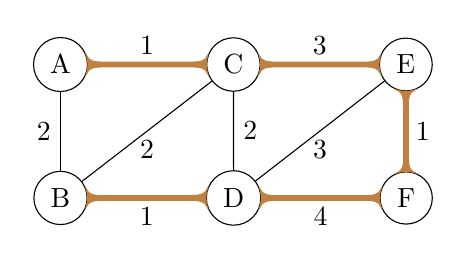
\begin{tikzpicture}[node distance = {1.0cm and 1.5cm}, 
  v/.style = {draw, circle},
  stv/.style = {v, fill = teal},	% vertices in spanning tree
  ste/.style = {circle connection bar, brown, fill}, % edges in spanning tree
]
  \node (a) [v] {A};
  \node (c) [v, right = of a] {C};
  \node (e) [v, right = of c] {E};

  \draw (a) to node[above] {1} (c);
  \draw (c) to node[above] {3} (e);

  \node (b) [v, below = of a] {B};
  \node (d) [v, right = of b] {D};
  \node (f) [v, right = of d] {F};

  \draw (b) to node[below] {1} (d);
  \draw (d) to node[below] {4} (f);

  \draw (a) to node[left] {2} (b);
  \draw (c) to node[below] {2} (b);
  \draw (c) to node[right] {2} (d);
  \draw (e) to node[below] {3} (d);
  \draw (e) to node[right] {1} (f);

  % \draw[ste] (a) to (b) to (c) to (d) to (e) to (f);
  \draw[ste] (a) to (c) to (e) to (f) to (d) to (b);
\end{tikzpicture}
\end{document}
